\chapter{INTRODUCTION}
\label{chp:1}
\section{Global Renewable Energy Status}
The share of the renewable energy systems has been reached significant levels. At the end of 2017, the renewable power capacity has reached 2179 GW throughout the world including hydro power plants \cite{InternationalRenewableEnergyAgencyIRENA2018}. Fig. \ref{renewablecap} shows the installed renewable energy capacity for leading countries at the end of 2016 and 2017. China has the biggest installed renewable energy capacity among these countries and increased its capacity by 73 GW in 2017.\par
\begin{figure}[h]
	\centering
	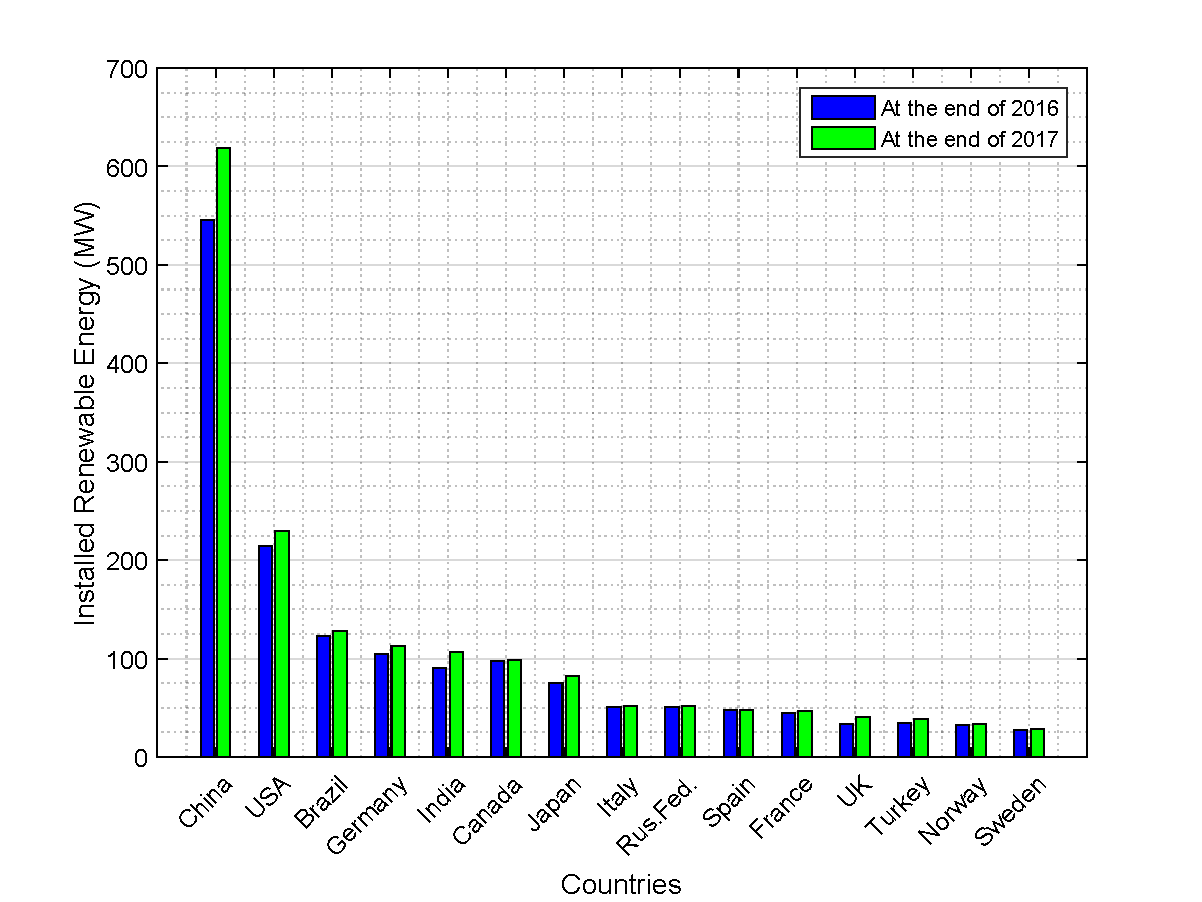
\includegraphics[scale=0.6]{renewablecapacities.pdf}
	\caption{Installed Renewable Energy Capacity of Leading Countries \cite{InternationalRenewableEnergyAgencyIRENA2018},\cite{InternationalRenewableEnergyAgency2017}}
	\label{renewablecap}
\end{figure}
EU countries promote the renewable energy systems from the very beginning. In 2008, two key main targets are set for 2020 by the European Council\cite{EuropeanCommission2008}: 
\begin{itemize}  
	\item At least 20 \% reduction in greenhouse gases (GHG) by 2020
	\item Achieving 20\% renewable energy share in energy consumption of EU by 2020
\end{itemize}
In order to accomplish these targets, the Renewable Energy Directive was published in 23 April 2009. This directive has set national binding targets for EU countries in order to accomplish the 20\% renewable energy target for EU and 10 \% target for the renewable energy usage in the transport \cite{EuropeanParliament2009}. In order to achieve the 20 \% target, each member state determined their own targets ranging from 10\% in Malta to 49\% in Sweden. According to the latest released report by Eurostat, renewable share of the EU in energy consumption has reached 17 \% in 2016 \cite{States2016}. Moreover, eleven of EU member states have already achieved their 2020 targets. Therefore, these ambitious targets imply that the increase in the renewable share will increase continuously.\par
Wind power has the highest share among the renewable energy sources in the installed renewable energy capacity except for hydro power. The wind power capacity at the end of 2017 has reached 514 GW worldwide\cite{InternationalRenewableEnergyAgencyIRENA2018}. The installed wind power capacity of the leading countries is shown in the Fig. \ref{windcap}. As in the case of total installed renewable energy capacity, China and USA have the highest installed capacities in the wind power capacity. \par
\begin{figure}[h!]
	\centering
	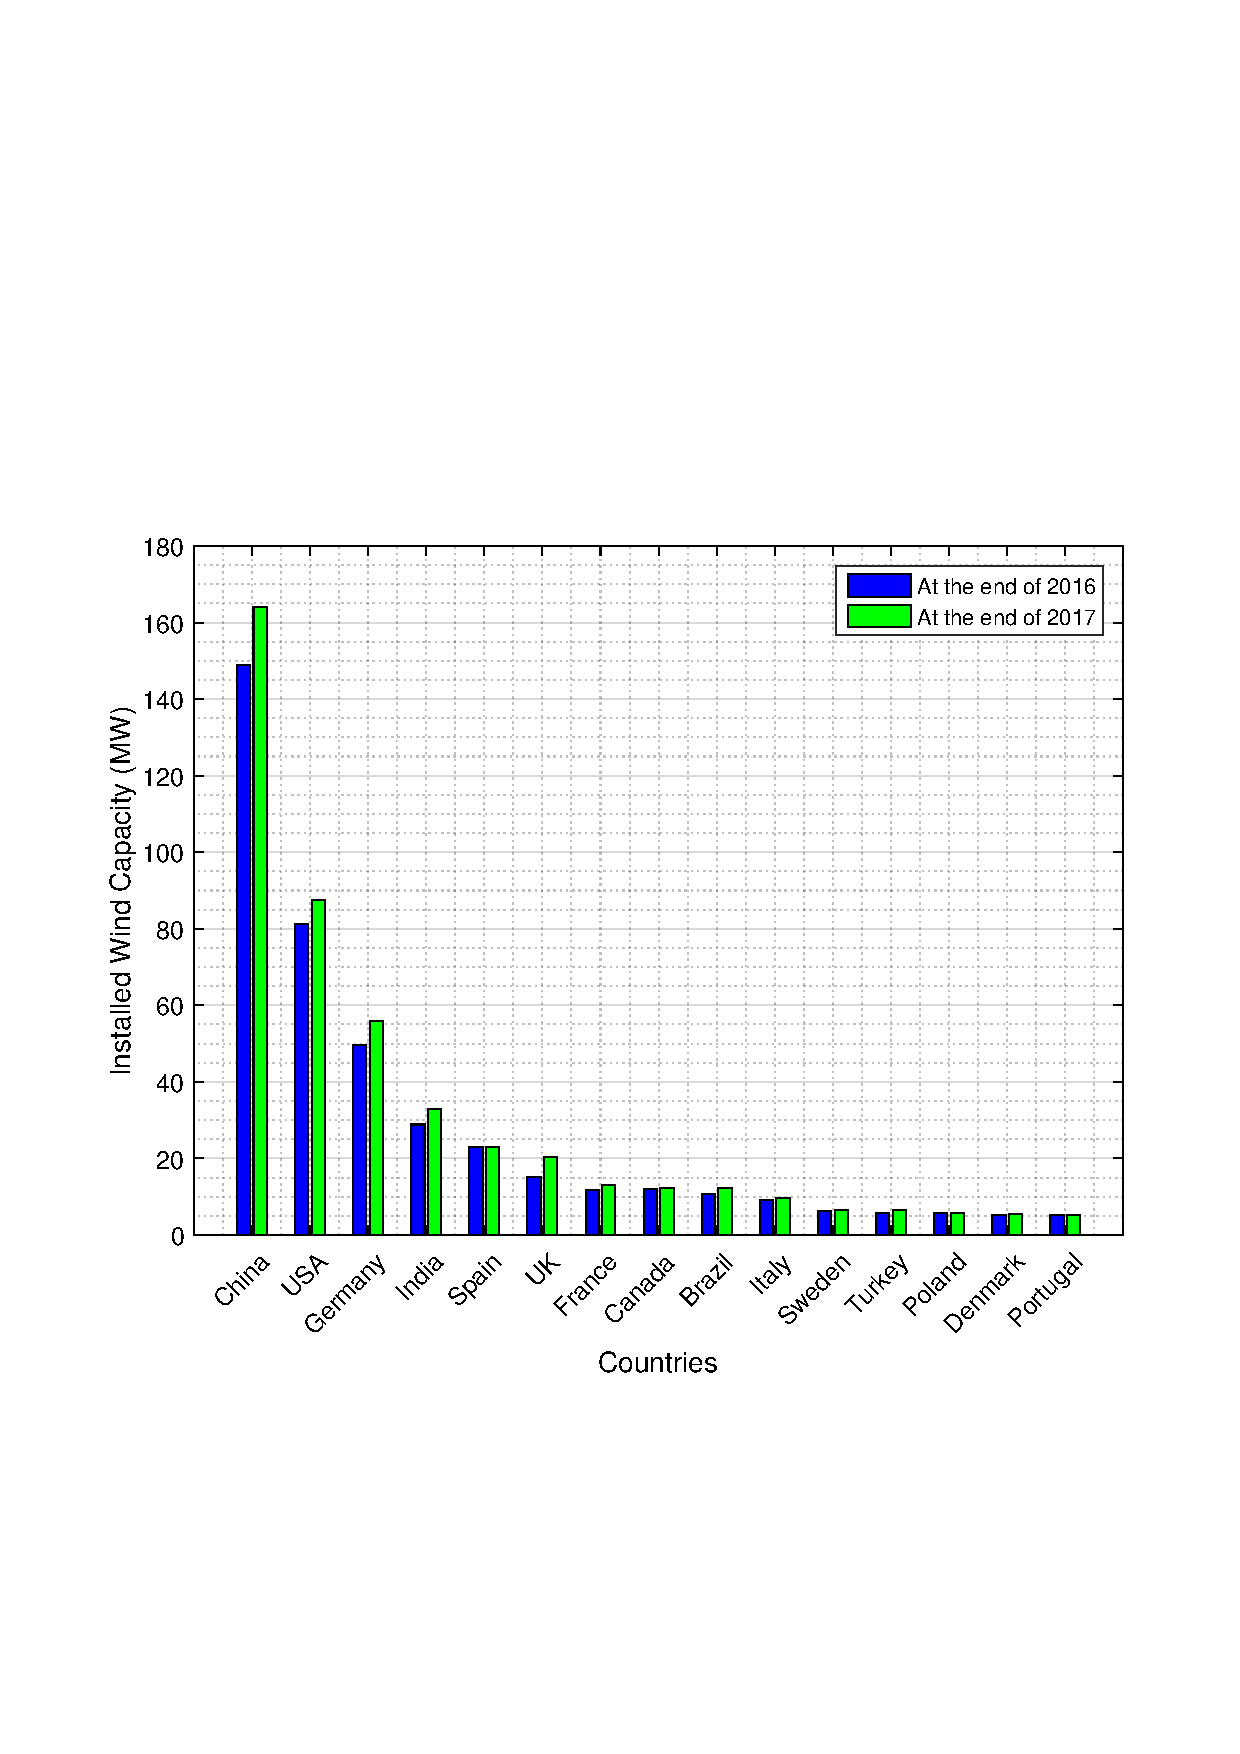
\includegraphics[scale=0.55]{windcapacity.pdf}
	\caption{Wind Power Capacity of Leading Countries in 2016 \cite{InternationalRenewableEnergyAgencyIRENA2018},\cite{InternationalRenewableEnergyAgency2017}}
	\label{windcap}
\end{figure}
The share of renewable energy is increasing continuously. Today, the discussion is about whether 100\% renewable energy is possible in the upcoming future. In \cite{REN212017d}, grid integration issues of wind and solar systems and the lack of sufficient storage technologies are considered as the main barrier for this target meanwhile the major problem seems as the existing energy industry. Nonetheless, a significant renewable share is expected even though the 100\% is realistic or not. The report published by IRENA (International Renewable Energy Agency) estimates the share of renewable energy in EU as 24\% by 2030 which is below proposed target of 27\%\cite{IRENA2014}. Nonetheless, the increase in the renewable energy share will continue in the upcoming future. \par
 
\section{Renewable Energy Problems}
It is an undeniable fact that renewable energy systems are advantageous in terms of global warming and carbon dioxide emission. Nonetheless, they also have disadvantages to the system operators due to intermittent energy generation profile. First of all, the term intermittent in the literature is related to the variable and uncontrollable nature of the renewable sources \cite{KlingeJacobsen2010}. Since the source of the Renewable Energy Sources (RES) is variable, it is not possible to adjust its output according to the demand. Therefore, the thermal plants have to be in the operation when high wind speeds and solar radiation exist. Moreover, the system requires additional start-ups and active power rise from partly loaded plants in order to balance the energy in the system because of the uncertainty of RES. These all create additional costs caused by high share of RES in the system \cite{Zipf2013}. Besides, power grid will face with transmission system issues as overloaded transmission lines, changes on the protection and control in the distribution system, greater level of power-factor control and low voltage ride-through (LVRT) requirements when the RES share is increased in the grid \cite{Ipakchi2009}.\par
Another challenge of increasing RES is the problem of power system frequency stability. Since the frequency of the power system depends on the balance between generation and consumption, grid operators are responsible for adjusting the generation in order to maintain a constant frequency. However, the renewable energy generation is strictly dependent on the renewable source i.e. solar radiation or wind speed. Therefore, renewable systems make the system operation harder due to their intermittent and uncertain power generation profiles. \par 
Frequency of the grid depends on the balance between supply and demand. As the balance is established, frequency stays constant. However, that is the ideal case. In fact, the load always varies. 
It is the responsibility of the grid operator to provide continues balance. Consequently, the grid frequency varies around the nominal frequency with small deviations. However, unintentional generation unit outages or instant load connections cause high deviations in the grid. A generic frequency disturbance is depicted in the Fig. \ref{freq2}. In the beginning of the disturbance, frequency falls with a slope that is called Rate of Change of Frequency (RoCoF) until the minimum frequency what is called frequency nadir is reached. Grid RoCoF is limited with the inertia of the generators. The higher grid inertia decreases RoCoF and increases the frequency nadir. \par
\begin{figure}[h!]
	\centering
	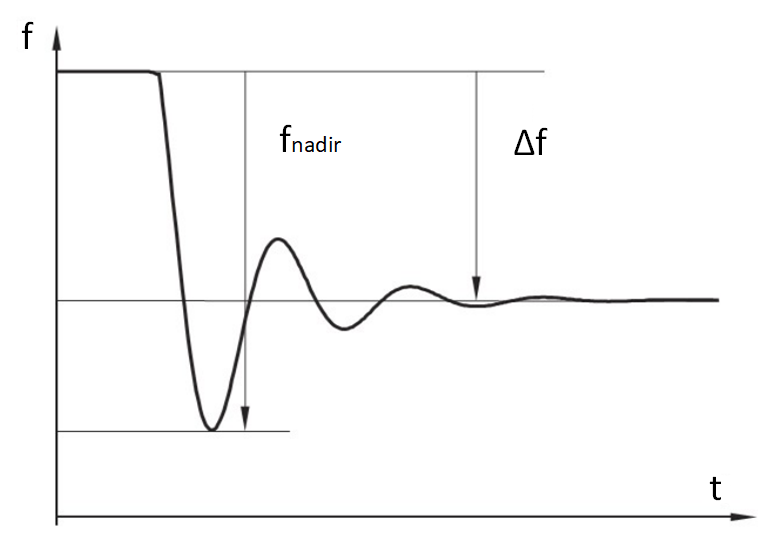
\includegraphics[scale=0.4]{freq2.png}
	\caption{A Generic Frequency Disturbance}
	\label{freq2}
\end{figure}
As the renewable systems with power electronics interface increase in the electricity grid, the grid equivalent inertia decreases. In \cite{Gautam2011}, the reduced grid inertia due to the high DFIG wind turbine penetration is emphasized. Moreover, the results of the reduced grid inertia following a disturbance are listed as: 
\begin{itemize}
	\item increased effective aggregated angular acceleration of synchronous machines which require high restoring forces
	\item high RoCoF and hence, decreased frequency nadir
\end{itemize}
It should be noted that this problem is not specific to DFIG wind turbines but renewable energy systems which are connected to the grid with power electronics. Conventional synchronous generators rotate at synchronous speed which is proportional to the grid frequency. If the grid frequency decreases, then the synchronous speed also decreases. In this case, the generator active power is increased inherently due to kinetic energy extraction from the generator inertia. The increase in active power provides action time for primary controllers and is crucial for frequency stability. \par
Different turbine topologies give different reactions to the frequency disturbances. Wind turbine generator topologies are shown in Fig. \ref{windtop}. Type-1 turbines are connected to grid with a asynchronous generator. The wind turbine generates active power as turbine rotates faster than synchronous speed. Therefore, the generator operates at the linear part of the torque-slip curve. Hence, the change in the grid frequency causes smaller decrease in the turbine speed. Type-2 is very similar to Type-1 except for the variable resistor which can shift the torque speed curve slightly. Hence, the frequency deviations affect the active power output of Type-1 and Type-2 \cite{Muljadi2012}. Type-3 wind turbines include Doubly-Fed Induction Generator (DFIG). DFIG stator is directly connected to grid meanwhile its rotor is connected to grid with a Partial Scale Power Converter (PSPC). Even though the stator is directly coupled to grid, the power electronics enable wind turbine to operate in a range of speeds. Therefore, the rotor frequency is also decoupled from grid.\par
\begin{figure}[h!]
	\centering
	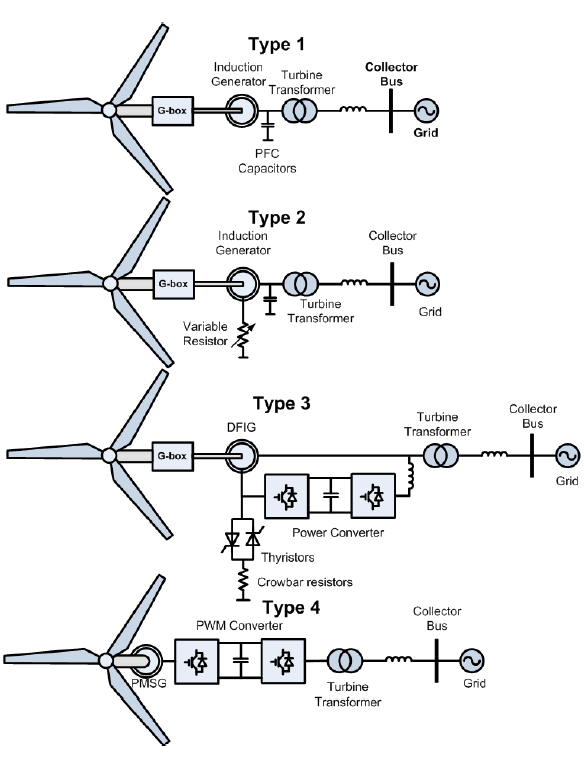
\includegraphics[scale=0.67]{windgentop.png}
	\caption{Wind Turbine Generator Configurations \cite{Muljadi2012}}
	\label{windtop}
\end{figure}
Type-4 wind turbines are connected to grid with back-to-back converters i.e. FSPC. AC/DC and DC/AC conversion decouples the grid frequency and the turbine speed. Due to the decoupling, Type-3 and Type-4 turbines can operate at the MPPT speed that capture the maximum power from air. Nonetheless, this results that Type-3 and 4 wind turbines are not affected from the grid frequency deviations. Therefore, these systems have no contribution to the grid inertia despite the fact that these systems include significant inertia. Hence, the aggregated grid inertia is reduced with the penetration of wind turbines with power electronics. The comparison for different types of generators is made in \cite{VanDeVyver2016} and listed in Table \ref{generatorcomparison}.\par  
\begin{table}[h]
	\centering
	\begin{tabular}{lc}
				\hline
		\multicolumn{1}{c}{\textbf{Type of the generator}}                                                                            & \textbf{Inertial Response Behaviur} \\ \hline
		Conventional Synchronous Generator                                                                                            & ++                                   \\
		Fixed Speed Induction Generator (FSIG)                                                                                        & +                                    \\
		Doubly Fed Induction Generator (DFIG)                                                                                         & -                                    \\
		\begin{tabular}[c]{@{}l@{}}Variable Speed Wind Turbine Generator\\ (Connected with Full Scale Power Electronics)\end{tabular} & None                                 \\ \hline
	\end{tabular}
	\caption{Comparison of Different Types of Generators for Inertial Response Behaviour}
	\label{generatorcomparison}
\end{table}
Another reason for the decrease in the grid inertia is the de-commitment or dispatch of the conventional sources due to economic concerns. Since the renewable energy systems have the lowest cost for energy production, they are preferred instead of conventional generators in the economical dispatch. As a result, conventional generators are dispatched to a lower generation profile or taken-off from operation.\par
It should be noted that grid inertia is directly related to the amount of load in the system in addition to the share of RES. Since the amount of online generators fluctuate within time, the grid aggregated inertia also changes. Hence, the scenario in which the system has low demand and also high renewable generation is the most critical one since the lowest grid inertia exists in the network.
\section{Literature Review}
Studies regarding inertial support date back to early 2000s. In the study \cite{Lalor2004}, the effect of the increasing wind energy penetration is investigated. The study concludes that increasing share of wind energy increases the primary reserve requirement for the successful grid operation. The increased frequency deviations, especially in light load conditions (high wind generation with low consumption scenario) can be mitigated in the system as long as the wind generation provides inertia support. Study in \cite{Ekanayake2003} states that DFIG wind turbines are decoupled from power system resulting in no contribution to system inertia. A supplementary loop is proposed for reinstating the machine inertia. Moreover, in \cite{Ekanayake2004}, performance of the  supplementary control loop is evaluated with the comparison of the inertial support of a fixed-speed wind turbine. The proposed control loop which is shown in Fig. \ref{inertiacontrol} is validated in \cite{Morren2006} and compared with the droop control in \cite{Morren2006a}.\par
\begin{figure}[h!]
	\centering
	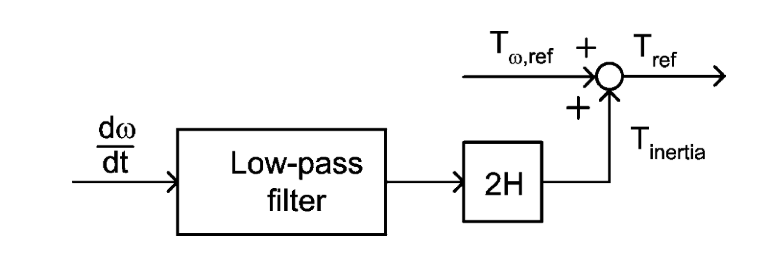
\includegraphics[width=.65\linewidth]{inertiacontrol.png}
	\caption{Inertia Controller in \cite{Morren2006a}}
	\label{inertiacontrol}
\end{figure}
It is an undeniable fact that renewable energy systems are the most economical way of producing electrical energy due to absence of any fuel cost. Therefore, they are to be operated in their rated power. If they are required for the primary frequency control, the wind turbine active power should be curtailed. In this way they can leave a margin for droop control. Droop control by wind energy systems is also studied in the literature. In \cite{Muljadi2012}, the inertial support of different types of wind turbines is compared. It is concluded that the Type-4 wind turbines are able to perform better performance for inertial support due to the power electronics interface. Moreover, combination of inertial support and droop control produces better results in these wind turbines.\par
Inertial support by utilizing the kinetic energy in the turbine is proposed in literature with two main methods. One of the methods is increasing the active power by a defined percentage and it is presented in literature with different names such as Fast
Inertial Support, Fast Power Reserve or Stepwise Inertial Control. In this type of support, the support power is released with a step increase in the active power. In \cite{Hansen2014}, the fast inertial support is proposed with predefined increases in the active power. Nevertheless, the converter ratings and the effect of the wind speed in the fast inertial support capability are not emphasized. \par
The second proposed method is the active power increase proportional to grid RoCoF. The method is called in literature as synthetic inertia control, hidden inertia control or
virtual inertia. Actually, synthetic inertia is a method not only for wind turbines but converter interfaced systems to emulate synchronous generators. In \cite{Zhu2013a}, the method is implemented a VSC-HVDC system in order to improve frequency stability of a weak grid. Study \cite{Hernandez2017} focuses on the implementation in the PV systems in coordination with energy storage systems. In \cite{Zhu2018a}, the synthetic inertia implementation is studied with cooperation with Lithium-Ion supercapacitors. \par
In the studies \cite{VanDeVyver2016},\cite{Conroy2008},\cite{Gonzalez-Longatt2013}, the synthetic inertia controller is implemented on a variable speed wind turbines. The active power output of the wind turbine is changed according to the grid RoCoF as shown in the Fig. \ref{inertiacontrol2}. The effects of the synthetic inertia implementation in a full-scale wind turbine are studied in \cite{Gonzalez-Longatt2013}. A variable synthetic inertia controller is proposed in \cite{Bonfiglio2019} that improves the speed recovery of the wind turbine. Nonetheless, the better speed recovery is achieved at the expense of the longer speed recovery time. \par
\begin{figure}[h!]
	\centering
	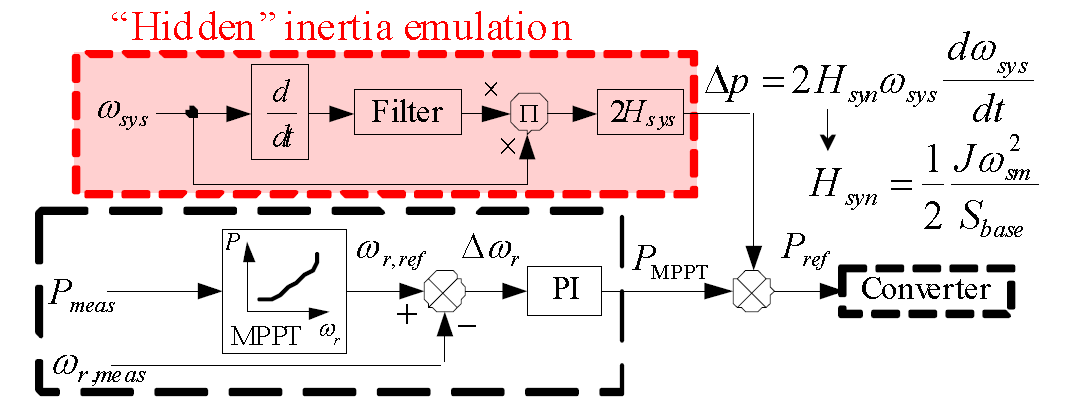
\includegraphics[width=.8\linewidth]{inertiacontrol2.png}
	\caption{Hidden Inertia Controller in\cite{Gonzalez-Longatt2013}}
	\label{inertiacontrol2}
\end{figure}
The modern wind turbine manufacturers also study the inertial support capability for their wind turbines. General Electrics has active power control module called as WindINERTIA for their wind turbines in order to react the large frequency disturbances. The control module can increase the power output of the wind turbine by 5-10\% for a few seconds (10\% for 15 seconds) \cite{Clark2009}. The control diagram of the module is shown in Fig. \ref{inertiacontrolge}. Moreover, Enercon provides inertial response capability to the turbines by allowing 10\% increase in the active power\cite{Enercon2018}. Nonetheless, solutions of GE and Enercon are independent of the grid RoCoF.\par
\begin{figure}[h!]
	\centering
	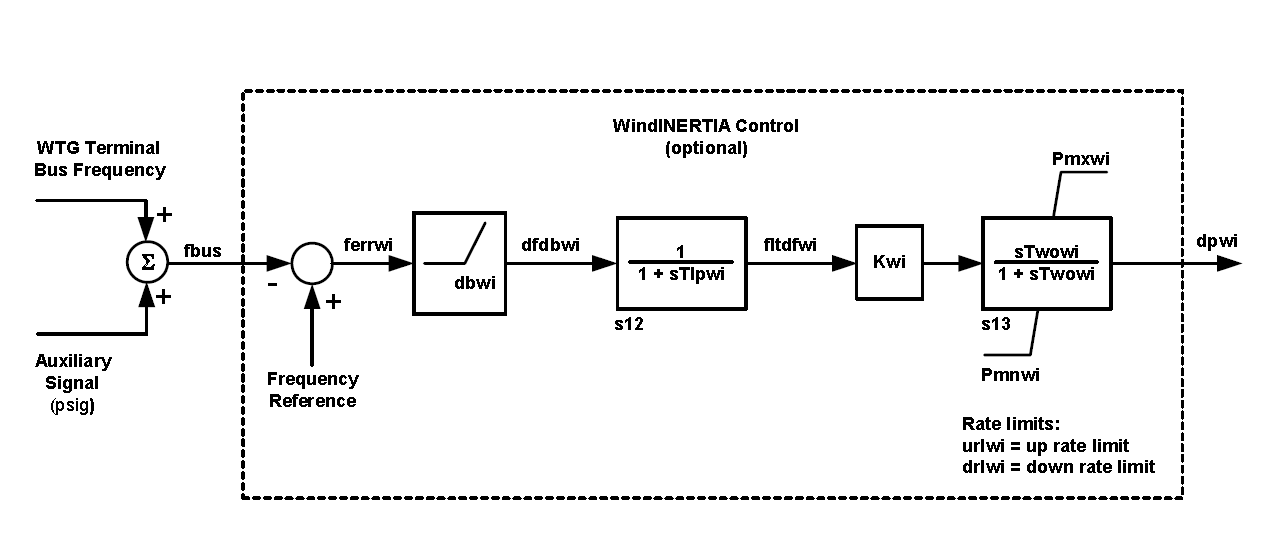
\includegraphics[width=.9\linewidth]{inertiacontrolge.png}
	\caption{GE WindINERTIA Control Diagram in \cite{Clark2009}}
	\label{inertiacontrolge}
\end{figure}
However, the full capacity of the wind turbines for inertial support is not studied in literature. Practical limits of the inertial support are studied in \cite{Gonzalez-Longatt2016} by varying the inertia constant to be emulated. The study focuses the emulation of higher inertia constants without consideration of the wind speed in the support time. The practical limits in terms of maximum achievable power and turbine internal parameters are not focused in the study. Finally, the studies in literature do not investigate the practical limits of the wind turbine. By investigating full capacity of the wind turbine, the importance of the wind turbines for frequency stability studies can be emphasized. 
\section{Thesis Motivation}
Although renewable energy systems are beneficial for environmental concerns and the absence of fuel cost, higher renewable penetration also brings operational challenges for system operators. One of the most important problems that comes with renewable energy is the power system frequency instability. With the high renewable penetration, grid aggregated inertia decreases. As a result, grid is exposed to high rate of change of frequency (RoCoF) for the disturbances. This implies that the successful operation of power systems with increasing renewable energy penetration is not achievable unless the decrease in the grid inertia is prevented. Therefore, the main objective of this study is to avoid the decrease in the grid inertia arising with the renewable energy penetration. In this way, the share of renewable energy systems can be increased without the negative effects on the power system operation.

%To avoid steeper frequency declines in the grid, all generation technologies should provide inertial support for the frequency disturbances.\par
Wind energy systems, especially variable speed wind turbines with full scale power electronics are the most promising renewable energy systems that can contribute to grid frequency stability due to the high inertia in their blades and generator and also their back-to-back converters that give ability to control its active power. Wind turbine with full-scale power electronics is the key solution to be used against the decrease in the grid inertia. However, the full capability of a wind turbine with full-scale power electronics has not been discovered yet. This study will explore the full capacity of the wind turbines for the inertial support. The practical limits of the wind turbines are explored under different wind speed scenarios. Another objective of this study is revealing the effects of grid supporting functions in the wind turbines. Besides, the differences between the frequency dependent and independent inertial support mechanisms are investigated especially for weak power systems.
%The knowledge of the wind turbine inertial support capability enables the grid operator to build new frequency regulating mechanisms. In this way, the participation of turbines for these mechanisms can be encouraged. \par
%Inertial support methods (either dependent on frequency or not) are presented in the literature. However, comparison of their performances under a weak power grid has not studied. This study aims to find out which type of inertial support is efficient for weak power grids. \par
%In Turkey, renewable energy systems produce electricity through the feed-in tariff that is the guaranteed price to these systems. Hence, the energy providers would not be volunteer for inertial support implementation unless system operators make this service mandatory or the implementation has economical benefits. The results of this thesis will present a basis for economical analysis by the energy provider perspective.
\section{Thesis Outline}
This thesis study focuses on the wind turbine inertial support limits and its effects on power system stability. The thesis starts with a brief summary of the renewable energy status in Chapter \ref{chp:1}. By reviewing the share of the renewable energy systems and the targets for upcoming future, the importance of the frequency stability studies is highlighted. Moreover, renewable energy problems and the proposed solutions in literature are presented. \par
In Chapter \ref{chp:2}, the frequency concept in power systems is extensively described. Since renewable energy systems are replaced or preferred over the conventional power generation units, the electricity grid is facing with frequency stability issues due to the absence of inertia-less units. Therefore, the behaviur of old-fashion power plants are described under frequency disturbances. Moreover, the frequency regulating mechanisms are presented. Finally, the energy markets are also explained in order to emphasize the position of renewable energy systems.\par
Chapter \ref{chp:3} presents the modelling of wind turbine used in this study. Since the existing variable speed wind turbines require modification in order to integrate to electricity grid, detailed modelling of these wind turbines is presented. By utilizing synthetic inertia method, a relation between grid frequency and the active power output is constructed.\par
The limits of the active power increase are investigated in Chapter \ref{chp:4}. The ability of increasing its active power output is already presented in literature. However, the limits of support power are studied for different wind speed scenarios. The real wind speed measurements from site are utilized to find the probability of support power for different wind speeds. Wind turbine inertial support limits and turbine internal parameters are observed for the non-dynamic frequency response.\par
Synthetic inertia implementation on a wind farm is studied in Chapter \ref{chp:5}. The effect of synthetic inertia is observed in a dynamic test case with renewable penetration. Test case is modified with different combinations in which the system is penetrated with wind farm with/without generator decommission are studied in this chapter. Frequency response of the test system is tested for different grid configurations as well as different emulated inertia constants. Furthermore, the synthetic inertia implementation is evaluated for the Turkish electricity system. \par
Chapter \ref{chp:6} evaluates the effects of the fast inertial support and synthetic inertia implementation. Moreover, an economical analysis from an energy provider perspective is given. Two hypothetical payment methods are constructed and compared to estimate which economical motive can convince the energy provider for participating grid supporting methods with renewable energy systems. \par
Chapter \ref{chp:7} presents a basic conclusion for the inertial support implementation which is either frequency dependent or not. The contribution of the thesis study on the grid inertia reduction is emphasized by reviewing the inertial support capability of the wind turbine especially for low and medium wind speeds. Moreover, the feasibility of the inertial support implementation is investigated in terms of the payment methods.

















